% Options for packages loaded elsewhere
\PassOptionsToPackage{unicode}{hyperref}
\PassOptionsToPackage{hyphens}{url}
%
\documentclass[
]{article}
\usepackage{lmodern}
\usepackage{amssymb,amsmath}
\usepackage{ifxetex,ifluatex}
\ifnum 0\ifxetex 1\fi\ifluatex 1\fi=0 % if pdftex
  \usepackage[T1]{fontenc}
  \usepackage[utf8]{inputenc}
  \usepackage{textcomp} % provide euro and other symbols
\else % if luatex or xetex
  \usepackage{unicode-math}
  \defaultfontfeatures{Scale=MatchLowercase}
  \defaultfontfeatures[\rmfamily]{Ligatures=TeX,Scale=1}
\fi
% Use upquote if available, for straight quotes in verbatim environments
\IfFileExists{upquote.sty}{\usepackage{upquote}}{}
\IfFileExists{microtype.sty}{% use microtype if available
  \usepackage[]{microtype}
  \UseMicrotypeSet[protrusion]{basicmath} % disable protrusion for tt fonts
}{}
\makeatletter
\@ifundefined{KOMAClassName}{% if non-KOMA class
  \IfFileExists{parskip.sty}{%
    \usepackage{parskip}
  }{% else
    \setlength{\parindent}{0pt}
    \setlength{\parskip}{6pt plus 2pt minus 1pt}}
}{% if KOMA class
  \KOMAoptions{parskip=half}}
\makeatother
\usepackage{xcolor}
\IfFileExists{xurl.sty}{\usepackage{xurl}}{} % add URL line breaks if available
\IfFileExists{bookmark.sty}{\usepackage{bookmark}}{\usepackage{hyperref}}
\hypersetup{
  hidelinks,
  pdfcreator={LaTeX via pandoc}}
\urlstyle{same} % disable monospaced font for URLs
\usepackage[margin=1in]{geometry}
\usepackage{color}
\usepackage{fancyvrb}
\newcommand{\VerbBar}{|}
\newcommand{\VERB}{\Verb[commandchars=\\\{\}]}
\DefineVerbatimEnvironment{Highlighting}{Verbatim}{commandchars=\\\{\}}
% Add ',fontsize=\small' for more characters per line
\usepackage{framed}
\definecolor{shadecolor}{RGB}{248,248,248}
\newenvironment{Shaded}{\begin{snugshade}}{\end{snugshade}}
\newcommand{\AlertTok}[1]{\textcolor[rgb]{0.94,0.16,0.16}{#1}}
\newcommand{\AnnotationTok}[1]{\textcolor[rgb]{0.56,0.35,0.01}{\textbf{\textit{#1}}}}
\newcommand{\AttributeTok}[1]{\textcolor[rgb]{0.77,0.63,0.00}{#1}}
\newcommand{\BaseNTok}[1]{\textcolor[rgb]{0.00,0.00,0.81}{#1}}
\newcommand{\BuiltInTok}[1]{#1}
\newcommand{\CharTok}[1]{\textcolor[rgb]{0.31,0.60,0.02}{#1}}
\newcommand{\CommentTok}[1]{\textcolor[rgb]{0.56,0.35,0.01}{\textit{#1}}}
\newcommand{\CommentVarTok}[1]{\textcolor[rgb]{0.56,0.35,0.01}{\textbf{\textit{#1}}}}
\newcommand{\ConstantTok}[1]{\textcolor[rgb]{0.00,0.00,0.00}{#1}}
\newcommand{\ControlFlowTok}[1]{\textcolor[rgb]{0.13,0.29,0.53}{\textbf{#1}}}
\newcommand{\DataTypeTok}[1]{\textcolor[rgb]{0.13,0.29,0.53}{#1}}
\newcommand{\DecValTok}[1]{\textcolor[rgb]{0.00,0.00,0.81}{#1}}
\newcommand{\DocumentationTok}[1]{\textcolor[rgb]{0.56,0.35,0.01}{\textbf{\textit{#1}}}}
\newcommand{\ErrorTok}[1]{\textcolor[rgb]{0.64,0.00,0.00}{\textbf{#1}}}
\newcommand{\ExtensionTok}[1]{#1}
\newcommand{\FloatTok}[1]{\textcolor[rgb]{0.00,0.00,0.81}{#1}}
\newcommand{\FunctionTok}[1]{\textcolor[rgb]{0.00,0.00,0.00}{#1}}
\newcommand{\ImportTok}[1]{#1}
\newcommand{\InformationTok}[1]{\textcolor[rgb]{0.56,0.35,0.01}{\textbf{\textit{#1}}}}
\newcommand{\KeywordTok}[1]{\textcolor[rgb]{0.13,0.29,0.53}{\textbf{#1}}}
\newcommand{\NormalTok}[1]{#1}
\newcommand{\OperatorTok}[1]{\textcolor[rgb]{0.81,0.36,0.00}{\textbf{#1}}}
\newcommand{\OtherTok}[1]{\textcolor[rgb]{0.56,0.35,0.01}{#1}}
\newcommand{\PreprocessorTok}[1]{\textcolor[rgb]{0.56,0.35,0.01}{\textit{#1}}}
\newcommand{\RegionMarkerTok}[1]{#1}
\newcommand{\SpecialCharTok}[1]{\textcolor[rgb]{0.00,0.00,0.00}{#1}}
\newcommand{\SpecialStringTok}[1]{\textcolor[rgb]{0.31,0.60,0.02}{#1}}
\newcommand{\StringTok}[1]{\textcolor[rgb]{0.31,0.60,0.02}{#1}}
\newcommand{\VariableTok}[1]{\textcolor[rgb]{0.00,0.00,0.00}{#1}}
\newcommand{\VerbatimStringTok}[1]{\textcolor[rgb]{0.31,0.60,0.02}{#1}}
\newcommand{\WarningTok}[1]{\textcolor[rgb]{0.56,0.35,0.01}{\textbf{\textit{#1}}}}
\usepackage{graphicx}
\makeatletter
\def\maxwidth{\ifdim\Gin@nat@width>\linewidth\linewidth\else\Gin@nat@width\fi}
\def\maxheight{\ifdim\Gin@nat@height>\textheight\textheight\else\Gin@nat@height\fi}
\makeatother
% Scale images if necessary, so that they will not overflow the page
% margins by default, and it is still possible to overwrite the defaults
% using explicit options in \includegraphics[width, height, ...]{}
\setkeys{Gin}{width=\maxwidth,height=\maxheight,keepaspectratio}
% Set default figure placement to htbp
\makeatletter
\def\fps@figure{htbp}
\makeatother
\setlength{\emergencystretch}{3em} % prevent overfull lines
\providecommand{\tightlist}{%
  \setlength{\itemsep}{0pt}\setlength{\parskip}{0pt}}
\setcounter{secnumdepth}{-\maxdimen} % remove section numbering

\author{}
\date{\vspace{-2.5em}}

\begin{document}

\hypertarget{reading}{%
\section{Reading in data locally and from the web}\label{reading}}

\hypertarget{overview}{%
\subsection{Overview}\label{overview}}

In this chapter, you'll learn to read spreadsheet-like data of various
formats into R from your local device and from the web. ``Reading'' (or
``loading'') is the process of converting data (stored as plain text, a
database, HTML, etc.) into an object (e.g., a dataframe) that R can
easily access and manipulate, and is thus the gateway to any data
analysis; you won't be able to analyze data unless you've loaded it
first. And because there are many ways to store data, there are
similarly many ways to read data into R. If you spend more time upfront
matching the data reading method to the type of data you have, you will
have to spend less time re-formatting, cleaning and wrangling your data
(the second step to all data analyses). It's like making sure your
shoelaces are tied well before going for a run so that you don't trip
later on!

\hypertarget{chapter-learning-objectives}{%
\subsection{Chapter learning
objectives}\label{chapter-learning-objectives}}

By the end of the chapter, students will be able to:

\begin{itemize}
\item
  define the following:

  \begin{itemize}
  \tightlist
  \item
    absolute file path
  \item
    relative file path
  \item
    url
  \end{itemize}
\item
  read data into R using a relative path and a url
\item
  compare and contrast the following functions:

  \begin{itemize}
  \tightlist
  \item
    \texttt{read\_csv}
  \item
    \texttt{read\_tsv}
  \item
    \texttt{read\_csv2}
  \item
    \texttt{read\_delim}
  \item
    \texttt{read\_excel}
  \end{itemize}
\item
  match the following \texttt{tidyverse} \texttt{read\_*} function
  arguments to their descriptions:

  \begin{itemize}
  \tightlist
  \item
    \texttt{file}
  \item
    \texttt{delim}
  \item
    \texttt{col\_names}
  \item
    \texttt{skip}
  \end{itemize}
\item
  choose the appropriate \texttt{tidyverse} \texttt{read\_*} function
  and function arguments to load a given plain text tabular data set
  into R
\item
  use \texttt{readxl} library's \texttt{read\_excel} function and
  arguments to load a sheet from an excel file into R
\item
  connect to a database using the \texttt{DBI} library's
  \texttt{dbConnect} function
\item
  list the tables in a database using the \texttt{DBI} library's
  \texttt{dbListTables} function
\item
  create a reference to a database table that is queriable using the
  \texttt{tbl} from the \texttt{dbplyr} library
\item
  retrieve data from a database query and bring it into R using the
  \texttt{collect} function from the \texttt{dbplyr} library
\item
  (\emph{optional}) scrape data from the web

  \begin{itemize}
  \tightlist
  \item
    read/scrape data from an internet URL using the rvest
    \texttt{html\_nodes} and \texttt{html\_text} functions
  \item
    compare downloading tabular data from a plain text file
    (e.g.~\texttt{.csv}) from the web versus scraping data from a
    \texttt{.html} file
  \end{itemize}
\end{itemize}

\hypertarget{absolute-and-relative-file-paths}{%
\subsection{Absolute and relative file
paths}\label{absolute-and-relative-file-paths}}

When you load a data set into R, you first need to tell R where that
files lives. The file could live on your computer (\emph{local}), or
somewhere on the internet (\emph{remote}). In this section we will
discuss the case where the file lives on your computer.

The place where the file lives on your computer is called the ``path''.
You can think of the path as directions to the file. There are two kinds
of paths: relative paths and absolute paths. A relative path is where
the file is in respect to where you currently are on the computer (e.g.,
where the Jupyter notebook file that you're working in is). On the other
hand, an absolute path is where the file is in respect to the base (or
root) folder of the computer's filesystem.

Suppose our computer's filesystem looks like the picture below, and we
are working in the Jupyter notebook titled
\texttt{worksheetk\_02.ipynb}. If we want to read in the \texttt{.csv}
file named \texttt{happiness\_report.csv} into our Jupyter notebook
using R, we could do this using either a relative or an absolute path.
We show what both choices below.

\textbf{Reading \texttt{happiness\_report.csv} using a relative path:}

\begin{verbatim}
happiness_data <- read_csv("data/happiness_report.csv")
\end{verbatim}

\textbf{Reading \texttt{happiness\_report.csv} using an absolute path:}

\begin{verbatim}
happiness_data <- read_csv("/home/jupyter/dsci-100/worksheet_02/data/happiness_report.csv")
\end{verbatim}

So which one should you use? Generally speaking, to ensure your code can
be run on a different computer, you should use relative paths (and it's
also less typing!). This is because the absolute path of a file (the
names of folders between the computer's root \texttt{/} and the file)
isn't usually the same across multiple computers. For example, suppose
Alice and Bob are working on a project together on the
\texttt{happiness\_report.csv} data. Alice's file is stored at

\texttt{/home/alice/project/data/happiness\_report.csv},

while Bob's is stored at

\texttt{/home/bob/project/data/happiness\_report.csv}.

Even though Alice and Bob stored their files in the same place on their
computers (in their home folders), the absolute paths are different due
to their different usernames. If Bob has code that loads the
\texttt{happiness\_report.csv} data using an absolute path, the code
won't work on Alice's computer. But the relative path from inside the
\texttt{project} folder (\texttt{data/happiness\_report.csv}) is the
same on both computers; any code that uses relative paths will work on
both!

See this video for another explanation:

\emph{Source:
\href{https://www.udacity.com/course/linux-command-line-basics--ud595}{Udacity
course ``Linux Command Line Basics''}}

\hypertarget{reading-tabular-data-from-a-plain-text-file-into-r}{%
\subsection{Reading tabular data from a plain text file into
R}\label{reading-tabular-data-from-a-plain-text-file-into-r}}

Now we will learn more about reading tabular data from a plain text file
into R, as well as how to write tabular data to a file. Last chapter we
learned about using the \texttt{tidyverse} \texttt{read\_csv} function
when reading files that match that functions expected defaults (column
names are present and commas are used as the delimiter/separator between
columns). In this section, we will learn how to read files do not
satisfy the default expectations of \texttt{read\_csv}.

Before we jump into the cases where the data aren't in the expected
default format for \texttt{tidyverse} and \texttt{read\_csv}, let's
revisit the simpler case where the defaults hold and the only argument
we need to give to the function is the path to the file,
\texttt{data/state\_property\_vote.csv}. We put \texttt{data/} before
the name of the file when we are loading the dataset because this
dataset is located in a sub-folder, named \texttt{data}, relative to
where we are running our R code.

Here is what the file would look in a plain text editor:

\begin{verbatim}
state,med_income,med_prop_val,population,mean_commute_minutes,party
AK,64222,197300,733375,10.46830207,Republican
AL,36924,94800,4830620,25.30990746,Republican
AR,35833,83300,2958208,22.40108933,Republican
AZ,44748,128700,6641928,20.58786,Republican
CA,53075,252100,38421464,23.38085172,Democrat
CO,48098,198900,5278906,19.50792188,Democrat
CT,69228,246450,3593222,24.349675,Democrat
DC,70848,475800,647484,28.2534,Democrat
DE,54976,228500,926454,24.45553333,Democrat
\end{verbatim}

And here is a review of how we can use \texttt{read\_csv} to load it
into R:

\begin{Shaded}
\begin{Highlighting}[]
\KeywordTok{library}\NormalTok{(tidyverse)}
\NormalTok{us\_data <{-}}\StringTok{ }\KeywordTok{read\_csv}\NormalTok{(}\StringTok{"data/state\_property\_vote.csv"}\NormalTok{)}
\NormalTok{us\_data}
\end{Highlighting}
\end{Shaded}

\begin{verbatim}
## # A tibble: 52 x 6
##    state med_income med_prop_val population mean_commute_minutes party     
##    <chr>      <dbl>        <dbl>      <dbl>                <dbl> <chr>     
##  1 AK         64222       197300     733375                 10.5 Republican
##  2 AL         36924        94800    4830620                 25.3 Republican
##  3 AR         35833        83300    2958208                 22.4 Republican
##  4 AZ         44748       128700    6641928                 20.6 Republican
##  5 CA         53075       252100   38421464                 23.4 Democrat  
##  6 CO         48098       198900    5278906                 19.5 Democrat  
##  7 CT         69228       246450    3593222                 24.3 Democrat  
##  8 DC         70848       475800     647484                 28.3 Democrat  
##  9 DE         54976       228500     926454                 24.5 Democrat  
## 10 FL         43355       125600   19645772                 24.8 Republican
## # … with 42 more rows
\end{verbatim}

\hypertarget{skipping-rows-when-reading-in-data}{%
\subsubsection{Skipping rows when reading in
data}\label{skipping-rows-when-reading-in-data}}

Often times information about how data was collected, or other relevant
information, is included at the top of the data file. This information
is usually written in sentence and paragraph form, with no delimiter
because it is not organized into columns. An example of this is shown
below:

\begin{verbatim}
Data source: https://datausa.io/
Record of how data was collected: https://github.com/UBC-DSCI/introduction-to-datascience/blob/master/data/src/retrieve_data_usa.ipynb
Date collected: 2017-06-06
state,med_income,med_prop_val,population,mean_commute_minutes,party
AK,64222,197300,733375,10.46830207,Republican
AL,36924,94800,4830620,25.30990746,Republican
AR,35833,83300,2958208,22.40108933,Republican
AZ,44748,128700,6641928,20.58786,Republican
CA,53075,252100,38421464,23.38085172,Democrat
CO,48098,198900,5278906,19.50792188,Democrat
CT,69228,246450,3593222,24.349675,Democrat
DC,70848,475800,647484,28.2534,Democrat
DE,54976,228500,926454,24.45553333,Democrat
\end{verbatim}

Using \texttt{read\_csv} as we did previously does not allow us to
correctly load the data into R. In the case of this file we end up only
reading in one column of the data set:

\begin{Shaded}
\begin{Highlighting}[]
\NormalTok{us\_data <{-}}\StringTok{ }\KeywordTok{read\_csv}\NormalTok{(}\StringTok{"data/state\_property\_vote\_meta{-}data.csv"}\NormalTok{)}
\end{Highlighting}
\end{Shaded}

\begin{verbatim}
## Parsed with column specification:
## cols(
##   `Data source: https://datausa.io/` = col_character()
## )
\end{verbatim}

\begin{Shaded}
\begin{Highlighting}[]
\NormalTok{us\_data}
\end{Highlighting}
\end{Shaded}

\begin{verbatim}
## # A tibble: 55 x 1
##    `Data source: https://datausa.io/`                                                                                      
##    <chr>                                                                                                                   
##  1 Record of how data was collected: https://github.com/UBC-DSCI/introduction-to-datascience/blob/master/data/src/retrieve…
##  2 Date collected: 2017-06-06                                                                                              
##  3 state                                                                                                                   
##  4 AK                                                                                                                      
##  5 AL                                                                                                                      
##  6 AR                                                                                                                      
##  7 AZ                                                                                                                      
##  8 CA                                                                                                                      
##  9 CO                                                                                                                      
## 10 CT                                                                                                                      
## # … with 45 more rows
\end{verbatim}

To successfully read data like this into R, the \texttt{skip} argument
can be useful to tell R how many lines to skip before it should start
reading in the data. In the example above, we would set this value to 3:

\begin{Shaded}
\begin{Highlighting}[]
\NormalTok{us\_data <{-}}\StringTok{ }\KeywordTok{read\_csv}\NormalTok{(}\StringTok{"data/state\_property\_vote\_meta{-}data.csv"}\NormalTok{, }\DataTypeTok{skip =} \DecValTok{3}\NormalTok{)}
\end{Highlighting}
\end{Shaded}

\begin{verbatim}
## Parsed with column specification:
## cols(
##   state = col_character(),
##   med_income = col_double(),
##   med_prop_val = col_double(),
##   population = col_double(),
##   mean_commute_minutes = col_double(),
##   party = col_character()
## )
\end{verbatim}

\begin{Shaded}
\begin{Highlighting}[]
\NormalTok{us\_data}
\end{Highlighting}
\end{Shaded}

\begin{verbatim}
## # A tibble: 52 x 6
##    state med_income med_prop_val population mean_commute_minutes party     
##    <chr>      <dbl>        <dbl>      <dbl>                <dbl> <chr>     
##  1 AK         64222       197300     733375                 10.5 Republican
##  2 AL         36924        94800    4830620                 25.3 Republican
##  3 AR         35833        83300    2958208                 22.4 Republican
##  4 AZ         44748       128700    6641928                 20.6 Republican
##  5 CA         53075       252100   38421464                 23.4 Democrat  
##  6 CO         48098       198900    5278906                 19.5 Democrat  
##  7 CT         69228       246450    3593222                 24.3 Democrat  
##  8 DC         70848       475800     647484                 28.3 Democrat  
##  9 DE         54976       228500     926454                 24.5 Democrat  
## 10 FL         43355       125600   19645772                 24.8 Republican
## # … with 42 more rows
\end{verbatim}

\hypertarget{read_delim-as-a-more-flexible-method-to-get-tabular-data-into-r}{%
\subsubsection{\texorpdfstring{\texttt{read\_delim} as a more flexible
method to get tabular data into
R}{read\_delim as a more flexible method to get tabular data into R}}\label{read_delim-as-a-more-flexible-method-to-get-tabular-data-into-r}}

When our tabular data comes in a different format, we can use the
\texttt{read\_delim} function instead. For example, a different version
of this same dataset has no column names and uses tabs as the delimiter
instead of commas.

Here is how the file would look in a plain text editor:

\begin{verbatim}
AK  64222   197300  733375  10.46830207 Republican
AL  36924   94800   4830620 25.30990746 Republican
AR  35833   83300   2958208 22.40108933 Republican
AZ  44748   128700  6641928 20.58786    Republican
CA  53075   252100  38421464    23.38085172 Democrat
CO  48098   198900  5278906 19.50792188 Democrat
CT  69228   246450  3593222 24.349675   Democrat
DC  70848   475800  647484  28.2534 Democrat
DE  54976   228500  926454  24.45553333 Democrat
FL  43355   125600  19645772    24.78055522 Republican
\end{verbatim}

To get this into R using the \texttt{read\_delim()} function, we specify
the first argument as the path to the file (as done with
\texttt{read\_csv}), and then provide values to the \texttt{delim}
argument (here a tab, which we represent by
\texttt{"\textbackslash{}t"}) and the \texttt{col\_names} argument (here
we specify that there are no column names be assigning it the value of
\texttt{FALSE}). Both \texttt{read\_csv()} and \texttt{read\_delim()}
have a \texttt{col\_names} argument and the default is \texttt{TRUE}.

\begin{Shaded}
\begin{Highlighting}[]
\NormalTok{us\_data <{-}}\StringTok{ }\KeywordTok{read\_delim}\NormalTok{(}\StringTok{"data/state\_property\_vote.tsv"}\NormalTok{,  }\DataTypeTok{delim =} \StringTok{"}\CharTok{\textbackslash{}t}\StringTok{"}\NormalTok{, }\DataTypeTok{col\_names =} \OtherTok{FALSE}\NormalTok{)}
\end{Highlighting}
\end{Shaded}

\begin{verbatim}
## Parsed with column specification:
## cols(
##   X1 = col_character(),
##   X2 = col_double(),
##   X3 = col_double(),
##   X4 = col_double(),
##   X5 = col_double(),
##   X6 = col_character()
## )
\end{verbatim}

\begin{Shaded}
\begin{Highlighting}[]
\NormalTok{us\_data}
\end{Highlighting}
\end{Shaded}

\begin{verbatim}
## # A tibble: 52 x 6
##    X1       X2     X3       X4    X5 X6        
##    <chr> <dbl>  <dbl>    <dbl> <dbl> <chr>     
##  1 AK    64222 197300   733375  10.5 Republican
##  2 AL    36924  94800  4830620  25.3 Republican
##  3 AR    35833  83300  2958208  22.4 Republican
##  4 AZ    44748 128700  6641928  20.6 Republican
##  5 CA    53075 252100 38421464  23.4 Democrat  
##  6 CO    48098 198900  5278906  19.5 Democrat  
##  7 CT    69228 246450  3593222  24.3 Democrat  
##  8 DC    70848 475800   647484  28.3 Democrat  
##  9 DE    54976 228500   926454  24.5 Democrat  
## 10 FL    43355 125600 19645772  24.8 Republican
## # … with 42 more rows
\end{verbatim}

Data frames in R need to have column names, thus if you read data into R
as a data frame without column names then R assigns column names for
them. If you used the \texttt{read\_*} functions to read the data into
R, then R gives each column a name of X1, X2, \ldots, XN, where N is the
number of columns in the data set.

\hypertarget{reading-tabular-data-directly-from-a-url}{%
\subsubsection{Reading tabular data directly from a
URL}\label{reading-tabular-data-directly-from-a-url}}

We can also use \texttt{read\_csv()} or \texttt{read\_delim()} (and
related functions) to read in tabular data directly from a url that
contains tabular data. In this case, we provide the url to
\texttt{read\_csv()} as the path to the file instead of a path to a
local file on our computer. Similar to when we specify a path on our
local computer, here we need to surround the url by quotes. All other
arguments that we use are the same as when using these functions with a
local file on our computer.

\begin{Shaded}
\begin{Highlighting}[]
\NormalTok{us\_data <{-}}\StringTok{ }\KeywordTok{read\_csv}\NormalTok{(}\StringTok{"https://raw.githubusercontent.com/UBC{-}DSCI/introduction{-}to{-}datascience/master/state\_property\_vote.csv"}\NormalTok{)}
\end{Highlighting}
\end{Shaded}

\begin{verbatim}
## Parsed with column specification:
## cols(
##   state = col_character(),
##   med_income = col_double(),
##   med_prop_val = col_double(),
##   population = col_double(),
##   mean_commute_minutes = col_double(),
##   party = col_character()
## )
\end{verbatim}

\begin{Shaded}
\begin{Highlighting}[]
\NormalTok{us\_data}
\end{Highlighting}
\end{Shaded}

\begin{verbatim}
## # A tibble: 52 x 6
##    state med_income med_prop_val population mean_commute_minutes party     
##    <chr>      <dbl>        <dbl>      <dbl>                <dbl> <chr>     
##  1 AK         64222       197300     733375                 10.5 Republican
##  2 AL         36924        94800    4830620                 25.3 Republican
##  3 AR         35833        83300    2958208                 22.4 Republican
##  4 AZ         44748       128700    6641928                 20.6 Republican
##  5 CA         53075       252100   38421464                 23.4 Democrat  
##  6 CO         48098       198900    5278906                 19.5 Democrat  
##  7 CT         69228       246450    3593222                 24.3 Democrat  
##  8 DC         70848       475800     647484                 28.3 Democrat  
##  9 DE         54976       228500     926454                 24.5 Democrat  
## 10 FL         43355       125600   19645772                 24.8 Republican
## # … with 42 more rows
\end{verbatim}

\hypertarget{previewing-a-data-file-before-reading-it-into-r}{%
\subsubsection{Previewing a data file before reading it into
R}\label{previewing-a-data-file-before-reading-it-into-r}}

In all the examples above, we gave you previews of the data file before
we read it into R. This is essential so that you can see whether or not
there are column names, what the delimiters are, and if there are lines
you need to skip. You should do this yourself when trying to read in
data files. In Jupyter, you preview data as a plain text file by
clicking on the file's name in the Jupyter home menu. We demonstrate
this in the video below:

\hypertarget{reading-data-from-an-microsoft-excel-file}{%
\subsection{Reading data from an Microsoft Excel
file}\label{reading-data-from-an-microsoft-excel-file}}

There are many other ways to store tabular datasets beyond plain text
files, and similarly many ways to load those datasets into R. For
example, it is very common to encounter, and need to load into R, data
stored as a Microsoft Excel spreadsheet (with the filename extension
\texttt{.xlsx}). To be able to do this, a key thing to know is that even
though \texttt{.csv} and \texttt{.xlsx} files look almost identical when
loaded into Excel, the data themselves are stored completely
differently. While \texttt{.csv} files are plain text files, where the
characters you see when you open the file in a text editor are exactly
the data they represent, this is not the case for \texttt{.xlsx} files.
Take a look at what a \texttt{.xlsx} file would look like in a text
editor:

\begin{verbatim}
,?'O
    _rels/.rels???J1??>E?{7?
<?V????w8?'J???'QrJ???Tf?d??d?o?wZ'?ф??@>?4'?|??hlIo??Fǟ
t                                                       8f??3wn
????t??u"/
          %~Ed2Ɩ??<?w??
                       ?Pd(??J-?E???7?'t(?-GZ?????y?ߎ??c~N?g[^_r?4
                                                                  yG?O
                                                                      ?K??G?RPX?<??,?'O[Content_Types].xml???n?0E%?J
                                                                                                                    ]TUE袏e??O??c[???????6q??s??d?m???ƻ\???H?^????3} ?rZY? ?:L60?^????‹?XTP+?|?3???"~?3T1W3???ޓ,?#p?R?!??w(??R???[S?D?kP?P!XS(?i?t?$?ei
оX?ܒa??4VT?,D?Jq
                D
                 ?????u?]??;??L?.8AhfNv}߼?hHF*җ??Jr?Q?%?g?U??CtX"8x>?.|????5j?/$???JE?c??~ݜ??4iw?????E;?+?S??w?cV+?:???2l???=?2nݡl?????;|?V??????c'?????9?P&Bcj,?'OdocProps/app.xml??1
                                                     ?0???k????A?u?U?]ȝ??{#?:;/<?g?Cߩd????M+?=???Z?O??R+??u?P?X?̔ KV@??M$??a???d,??_???4??5v?R????9D????t??Fk?Ú'P?=?,?'OdocProps/core.xml??MO?0
                                                             ??J?{???3j?h'??(q??U4J
                                                                                   ??=i?I'?b??[v?ޙ!??{gk?
                                                                                                         F2????v5yj7??"J???,?d???J???C??ƚl??4?-?$ۤ??`$?4t?K?.;?%c?J-Q҉??G<??ɑZ-H????
                                                  X????z???6?????~q??X??ٗ6?????q^>??tH???*?D???M?g
??D?????????ݐ?d?:g).ے?3.??׉uԟ?ǟj?P?F؝,?'Oxl/_rels/workbook.xml.rels??Ak1??J?{7???R?^J?kk@Hf7??I?L???E]A?Þ?{a??`f?????b?6xUQ?@o?m}??o????X{???Q?????;?y?\?
                        O
?YY??4΀?L??S??k?252j??
??V ?C?g?C]???????
?
???E??TENyf6%
             ?Y????|??:%???}^ N?Q?ۤ?N'????)??F?\??P?G??,?'O'xl/printerSettings/printerSettings1.bin?Wmn? 
                                                                                                        ??Sp>?G???q?#
                                                                                                                     ?I??ڒ5R'???q????(?L
??m??8F?5<  L`?ݍ-?`?A??2{dp??9R#?>7??Xu???ꋝ/?X??HI?|?
                                                          ??r)???\?VA8?2dFfq???I]]o
5`??<͘??6uA ?
\end{verbatim}

This type of file representation allows Excel files to store additional
things that you cannot store in a \texttt{.csv} file, such as fonts,
text formatting, graphics, multiple sheets and more. And despite looking
odd in a plain text editor, we can read Excel spreadsheets into R using
the \texttt{readxl} package developed specifically for this purpose.

\begin{Shaded}
\begin{Highlighting}[]
\KeywordTok{library}\NormalTok{(readxl)}
\NormalTok{us\_data <{-}}\StringTok{ }\KeywordTok{read\_excel}\NormalTok{(}\StringTok{"data/state\_property\_vote.xlsx"}\NormalTok{)}
\NormalTok{us\_data}
\end{Highlighting}
\end{Shaded}

\begin{verbatim}
## # A tibble: 52 x 6
##    state med_income med_prop_val population mean_commute_minutes party     
##    <chr>      <dbl>        <dbl>      <dbl>                <dbl> <chr>     
##  1 AK         64222       197300     733375                 10.5 Republican
##  2 AL         36924        94800    4830620                 25.3 Republican
##  3 AR         35833        83300    2958208                 22.4 Republican
##  4 AZ         44748       128700    6641928                 20.6 Republican
##  5 CA         53075       252100   38421464                 23.4 Democrat  
##  6 CO         48098       198900    5278906                 19.5 Democrat  
##  7 CT         69228       246450    3593222                 24.3 Democrat  
##  8 DC         70848       475800     647484                 28.3 Democrat  
##  9 DE         54976       228500     926454                 24.5 Democrat  
## 10 FL         43355       125600   19645772                 24.8 Republican
## # … with 42 more rows
\end{verbatim}

If the \texttt{.xlsx} file has multiple sheets, then you have to use the
\texttt{sheet} argument to specify either the sheet number or name. You
can also specify cell ranges using the \texttt{range} argument. This is
useful in cases where a single sheet contains multiple tables (a sad
thing that happens to many Excel spreadsheets).

As with plain text files, you should always try to explore the data file
before importing it into R. This helps you decide which arguments you
need to use to successfully load the data into R. If you do not have the
Excel program on your computer, there are other free programs you can
use to preview the file. Examples include Google Sheets and Libre
Office.

\hypertarget{reading-data-from-a-database}{%
\subsection{Reading data from a
database}\label{reading-data-from-a-database}}

Another very common form of data storage to be read into R for the
purpose of data analysis is the relational database. There are many
relational database management systems, such as SQLite, MySQL,
PosgreSQL, Oracle, and many more. Almost all employ SQL
(\emph{structured query language}) to pull data from the database.
Thankfully, you don't need to know SQL to analyze data from a database;
several packages have been written that allow R to connect to relational
databases and use the R programming language as the front end (what the
user types in) to pull data from them. In this book we will give
examples of how to do this using R with SQLite and PostgreSQL databases.

\hypertarget{reading-data-from-a-sqlite-database}{%
\subsubsection{Reading data from a SQLite
database}\label{reading-data-from-a-sqlite-database}}

SQLite is probably the simplest relational database that one can use in
combination with R. SQLite databases are self-contained and usually
stored and accessed locally on one computer. Data is usually stored in a
file with a \texttt{.db} extension. Similar to Excel files, these are
not plain text files and cannot be read in a plain text editor.

The first thing you need to do to read data into R from a database is to
connect to the database. We do that using the \texttt{dbConnect}
function from the \texttt{DBI} (database interface) package. This does
not read in the data, but simply tells R where the database is and opens
up a communication channel.

\begin{Shaded}
\begin{Highlighting}[]
\KeywordTok{library}\NormalTok{(DBI)}
\NormalTok{con\_state\_data <{-}}\StringTok{ }\KeywordTok{dbConnect}\NormalTok{(RSQLite}\OperatorTok{::}\KeywordTok{SQLite}\NormalTok{(), }\StringTok{"data/state\_property\_vote.db"}\NormalTok{)}
\end{Highlighting}
\end{Shaded}

Often times relational databases have many tables, and their power comes
from the useful ways they can be joined. Thus anytime you want to access
data from a relational database you need to know the table names. You
can get the names of all the tables in the database using the
\texttt{dbListTables} function:

\begin{Shaded}
\begin{Highlighting}[]
\NormalTok{tables <{-}}\StringTok{ }\KeywordTok{dbListTables}\NormalTok{(con\_state\_data)}
\NormalTok{tables}
\end{Highlighting}
\end{Shaded}

\begin{verbatim}
## [1] "state"
\end{verbatim}

We only get one table name returned form calling \texttt{dbListTables},
and this tells us that there is only one table in this database. To
reference a table in the database so we can do things like select
columns and filter rows, we use the \texttt{tbl} function from the
\texttt{dbplyr} package:

\begin{Shaded}
\begin{Highlighting}[]
\KeywordTok{library}\NormalTok{(dbplyr)}
\NormalTok{state\_db <{-}}\StringTok{ }\KeywordTok{tbl}\NormalTok{(con\_state\_data, }\StringTok{"state"}\NormalTok{)}
\NormalTok{state\_db}
\end{Highlighting}
\end{Shaded}

\begin{verbatim}
## # Source:   table<state> [?? x 6]
## # Database: sqlite 3.29.0 [/Users/tiffany/Documents/ubc-dsci/introduction-to-datascience/data/state_property_vote.db]
##    state med_income med_prop_val population mean_commute_minutes party     
##    <chr>      <dbl>        <dbl>      <dbl>                <dbl> <chr>     
##  1 AK         64222       197300     733375                 10.5 Republican
##  2 AL         36924        94800    4830620                 25.3 Republican
##  3 AR         35833        83300    2958208                 22.4 Republican
##  4 AZ         44748       128700    6641928                 20.6 Republican
##  5 CA         53075       252100   38421464                 23.4 Democrat  
##  6 CO         48098       198900    5278906                 19.5 Democrat  
##  7 CT         69228       246450    3593222                 24.3 Democrat  
##  8 DC         70848       475800     647484                 28.3 Democrat  
##  9 DE         54976       228500     926454                 24.5 Democrat  
## 10 FL         43355       125600   19645772                 24.8 Republican
## # … with more rows
\end{verbatim}

Although it looks like we just got a data frame from the database, we
didn't! It's a \emph{reference}, showing us data that is still in the
SQLite database (note the first two lines of the output). It does this
because databases are often more efficient at selecting, filtering and
joining large datasets than R. And typically, the database will not even
be stored on your computer, but rather a more powerful machine somewhere
on the web. So R is lazy and waits to bring this data into memory until
you explicitly tell it to do so using the \texttt{collect} function from
the \texttt{dbplyr} library.

Here we will filter for only states that voted for the Republican
candidate in the 2016 Presidential election, and then use
\texttt{collect} to finally bring this data into R as a data frame.

\begin{Shaded}
\begin{Highlighting}[]
\NormalTok{republican\_db <{-}}\StringTok{ }\KeywordTok{filter}\NormalTok{(state\_db, party }\OperatorTok{==}\StringTok{ "Republican"}\NormalTok{)}
\NormalTok{republican\_db}
\end{Highlighting}
\end{Shaded}

\begin{verbatim}
## # Source:   lazy query [?? x 6]
## # Database: sqlite 3.29.0 [/Users/tiffany/Documents/ubc-dsci/introduction-to-datascience/data/state_property_vote.db]
##    state med_income med_prop_val population mean_commute_minutes party     
##    <chr>      <dbl>        <dbl>      <dbl>                <dbl> <chr>     
##  1 AK        64222        197300     733375                 10.5 Republican
##  2 AL        36924         94800    4830620                 25.3 Republican
##  3 AR        35833         83300    2958208                 22.4 Republican
##  4 AZ        44748        128700    6641928                 20.6 Republican
##  5 FL        43355        125600   19645772                 24.8 Republican
##  6 GA        37865        101700   10006693                 24.5 Republican
##  7 IA        49448        102700    3093526                 18.4 Republican
##  8 ID        43080.       143900    1616547                 19.9 Republican
##  9 IN        47194        111800    6568645                 23.5 Republican
## 10 KS        46875         85200    2892987                 16.7 Republican
## # … with more rows
\end{verbatim}

\begin{Shaded}
\begin{Highlighting}[]
\NormalTok{republican\_data <{-}}\StringTok{ }\KeywordTok{collect}\NormalTok{(republican\_db)}
\NormalTok{republican\_data}
\end{Highlighting}
\end{Shaded}

\begin{verbatim}
## # A tibble: 31 x 6
##    state med_income med_prop_val population mean_commute_minutes party     
##    <chr>      <dbl>        <dbl>      <dbl>                <dbl> <chr>     
##  1 AK        64222        197300     733375                 10.5 Republican
##  2 AL        36924         94800    4830620                 25.3 Republican
##  3 AR        35833         83300    2958208                 22.4 Republican
##  4 AZ        44748        128700    6641928                 20.6 Republican
##  5 FL        43355        125600   19645772                 24.8 Republican
##  6 GA        37865        101700   10006693                 24.5 Republican
##  7 IA        49448        102700    3093526                 18.4 Republican
##  8 ID        43080.       143900    1616547                 19.9 Republican
##  9 IN        47194        111800    6568645                 23.5 Republican
## 10 KS        46875         85200    2892987                 16.7 Republican
## # … with 21 more rows
\end{verbatim}

Why bother to use the \texttt{collect} function? The data looks pretty
similar in both outputs shown above. And \texttt{dbplyr} provides lots
of functions similar to \texttt{filter} that you can use to directly
feed the database reference (what \texttt{tbl} gives you) into
downstream analysis functions (e.g., \texttt{ggplot2} for data
visualization and \texttt{lm} for linear regression modeling). However,
this does not work in \emph{every} case; look what happens when we try
to use \texttt{nrow} to count rows in a data frame:

\begin{Shaded}
\begin{Highlighting}[]
\KeywordTok{nrow}\NormalTok{(republican\_db)}
\end{Highlighting}
\end{Shaded}

\begin{verbatim}
## [1] NA
\end{verbatim}

or \texttt{tail} to preview the last 6 rows of a data frame:

\begin{verbatim}
tail(republican_db)
\end{verbatim}

\begin{verbatim}
## Error: tail() is not supported by sql sources
\end{verbatim}

Additionally, some operations will not work to extract columns or single
values from the reference given by the \texttt{tbl} function. Thus, once
you have finished your data wrangling of the \texttt{tbl} database
reference object, it is advisable to then bring it into your local
machine's memory using \texttt{collect} as a data frame.

\hypertarget{reading-data-from-a-postgresql-database}{%
\subsubsection{Reading data from a PostgreSQL
database}\label{reading-data-from-a-postgresql-database}}

PostgreSQL (also called Postgres) is a very popular free and open-source
option for relational database software. Unlike SQLite, PostgreSQL uses
a client--server database engine, as it was designed to be used and
accessed on a network. This means that you have to provide more
information to R when connecting to Postgres databases. The additional
information that you need to include when you call the
\texttt{dbConnect} function is listed below:

\begin{itemize}
\tightlist
\item
  \texttt{dbname} - the name of the database (a single PostgreSQL
  instance can host more than one database)
\item
  \texttt{host} - the URL pointing to where the database is located
\item
  \texttt{port} - the communication endpoint between R and the
  PostgreSQL database (this is typically 5432 for PostgreSQL)
\item
  \texttt{user} - the username for accessing the database
\item
  \texttt{password} - the password for accessing the database
\end{itemize}

Additionally, we must use the \texttt{RPostgres} library instead of
\texttt{RSQLite} in the \texttt{dbConnect} function call. Below we
demonstrate how to connect to a version of the \texttt{can\_mov\_db}
database, which contains information about Canadian movies (\emph{note -
this is a synthetic, or artificial, database}).

\begin{verbatim}
library(RPostgres)
can_mov_db_con <- dbConnect(RPostgres::Postgres(), dbname = "can_mov_db",
                        host = "r7k3-mds1.stat.ubc.ca", port = 5432,
                        user = "user0001", password = '################')
\end{verbatim}

After opening the connection, everything looks and behaves almost
identically to when we were using an SQLite database in R. For example,
we can again use \texttt{dbListTables} to find out what tables are in
the \texttt{can\_mov\_db} database:

\begin{verbatim}
dbListTables(can_mov_db_con)
\end{verbatim}

\begin{verbatim}
 [1] "themes"            "medium"           "titles"     "title_aliases"       "forms"            
 [6] "episodes"          "names"      "names_occupations" "occupation"       "ratings" 
\end{verbatim}

We see that there are 10 tables in this database. Let's first look at
the \texttt{"ratings"} table to find the lowest rating that exists in
the \texttt{can\_mov\_db} database:

\begin{verbatim}
ratings_db <- tbl(can_mov_db_con, "ratings")
ratings_db
\end{verbatim}

\begin{verbatim}
# Source:   table<ratings> [?? x 3]
# Database: postgres [user0001@r7k3-mds1.stat.ubc.ca:5432/can_mov_db]
   title              average_rating num_votes
   <chr>                    <dbl>     <int>
 1 The Grand Seduction       6.6       150
 2 Rhymes for Young Ghouls   6.3      1685
 3 Mommy                     7.5      1060
 4 Incendies                 6.1      1101
 5 Bon Cop, Bad Cop          7.0       894
 6 Goon                      5.5      1111
 7 Monsieur Lazhar           5.6       610
 8 What if                   5.3      1401
 9 The Barbarian Invations   5.8        99
10 Away from Her             6.9      2311
# … with more rows
\end{verbatim}

To find the lowest rating that exists in the data base, we first need to
extract the \texttt{average\_rating} column using \texttt{select}:

\begin{verbatim}
avg_rating_db <- select(ratings_db, average_rating)
avg_rating_db
\end{verbatim}

\begin{verbatim}
# Source:   lazy query [?? x 1]
# Database: postgres [user0001@r7k3-mds1.stat.ubc.ca:5432/can_mov_db]
   average_rating
            <dbl>
 1            6.6
 2            6.3
 3            7.5
 4            6.1
 5            7.0
 6            5.5
 7            5.6
 8            5.3
 9            5.8
10            6.9
# … with more rows
\end{verbatim}

Next we use \texttt{min} to find the minimum rating in that column:

\begin{verbatim}
min(avg_rating_db)
\end{verbatim}

\begin{verbatim}
Error in min(avg_rating_db) : invalid 'type' (list) of argument
\end{verbatim}

Instead of the minimum, we get an error! This is another example of when
we need to use the \texttt{collect} function to bring the data into R
for further computation:

\begin{verbatim}
avg_rating_data <- collect(avg_rating_db)
min(avg_rating_data)
\end{verbatim}

\begin{verbatim}
[1] 1
\end{verbatim}

We see the lowest rating given to a movie is 1, indicating that it must
have been a really bad movie\ldots{}

\hypertarget{writing-data-from-r-to-a-.csv-file}{%
\subsection{\texorpdfstring{Writing data from R to a \texttt{.csv}
file}{Writing data from R to a .csv file}}\label{writing-data-from-r-to-a-.csv-file}}

At the middle and end of a data analysis, we often want to write a data
frame that has changed (either through filtering, selecting, mutating or
summarizing) to a file so that we can share it with others or use it for
another step in the analysis. The most straightforward way to do this is
to use the \texttt{write\_csv} function from the \texttt{tidyverse}
library. The default arguments for this file are to use a comma
(\texttt{,}) as the delimiter and include column names. Below we
demonstrate creating a new version of the US state-level property,
income, population and voting data from 2015 and 2016 that does not
contain the territory of Puerto Rico, and then writing this to a
\texttt{.csv} file:

\begin{Shaded}
\begin{Highlighting}[]
\NormalTok{state\_data <{-}}\StringTok{ }\KeywordTok{filter}\NormalTok{(us\_data, state }\OperatorTok{!=}\StringTok{ "PR"}\NormalTok{)}
\KeywordTok{write\_csv}\NormalTok{(state\_data, }\StringTok{"data/us\_states\_only.csv"}\NormalTok{)}
\end{Highlighting}
\end{Shaded}

\hypertarget{scraping-data-off-the-web-using-r}{%
\subsection{Scraping data off the web using
R}\label{scraping-data-off-the-web-using-r}}

In the first part of this chapter we learned how to read in data from
plain text files that are usually ``rectangular'' in shape using the
tidyverse \texttt{read\_*} functions. Sadly, not all data comes in this
simple format, but happily there are many other tools we can use to read
in more messy/wild data formats. One common place people often want/need
to read in data from is websites. Such data exists in an a
non-rectangular format. One quick and easy solution to get this data is
to copy and paste it, however this becomes painstakingly long and boring
when there is a lot of data that needs gathering, and anytime you start
doing a lot of copying and pasting it is very likely you will introduce
errors.

The formal name for gathering non-rectangular data from the web and
transforming it into a more useful format for data analysis is
\textbf{web scraping}. There are two different ways to do web scraping:
1) screen scraping (similar to copying and pasting from a website, but
done in a programmatic way to minimize errors and maximize efficiency)
and 2) web APIs (\textbf{a}pplication \textbf{p}rogramming
\textbf{i}nterface) (a website that provides a programatic way of
returning the data as JSON or XML files via http requests). In this
course we will explore the first method, screen scraping using R's
\href{https://github.com/hadley/rvest}{\texttt{rvest} package}.

\hypertarget{html-and-css-selectors}{%
\subsubsection{HTML and CSS selectors}\label{html-and-css-selectors}}

Before we jump into scraping, let's set up some motivation and learn a
little bit about what the ``source code'' of a website looks like. Say
we are interested in knowing the average rental price (per square
footage) of the most recently available 1 bedroom apartments in
Vancouver from \url{https://vancouver.craigslist.org}. When we visit the
Vancouver Craigslist website and search for 1 bedroom apartments, this
is what we are shown:

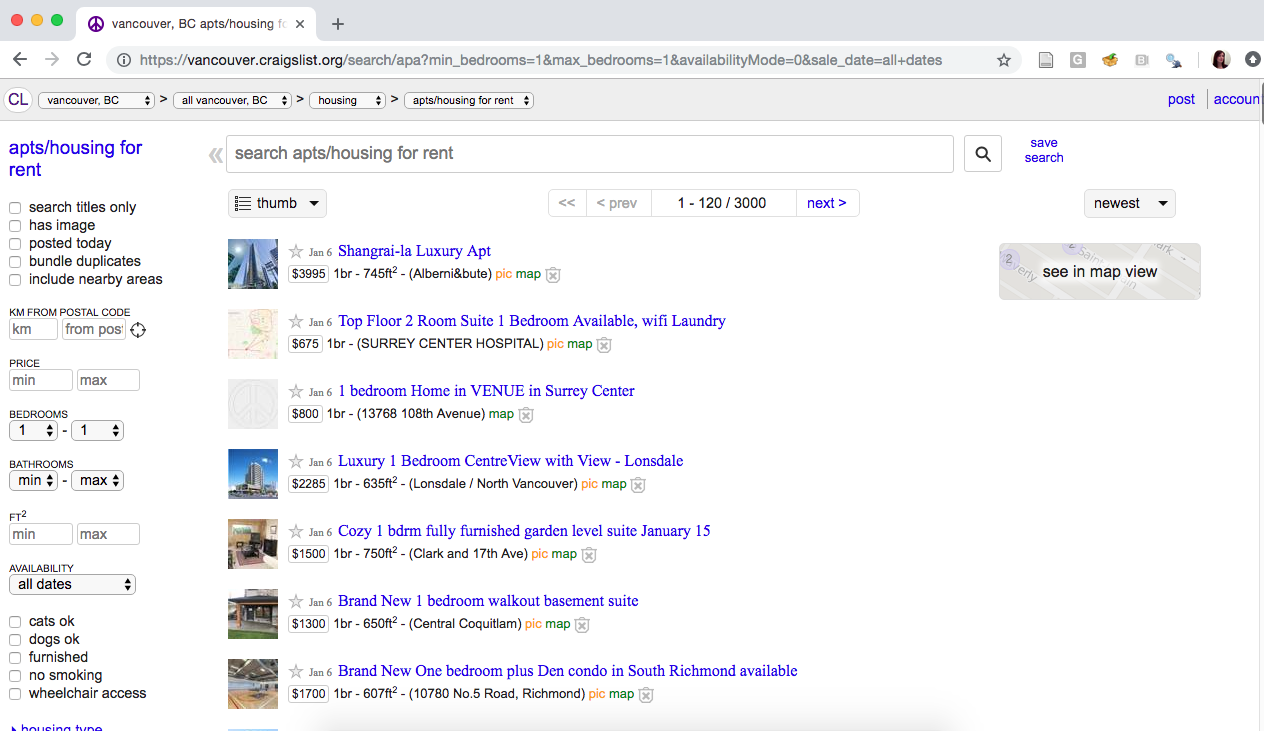
\includegraphics{img/craigslist_human.png}

From that page, it's pretty easy for our human eyes to find the
apartment price and square footage. But how can we do this
programmatically so we don't have to copy and paste all these numbers?
Well, we have to deal with the webpage source code, which we show a
snippet of below (and link to the \href{img/website_source.txt}{entire
source code here}):

\begin{verbatim}
        <span class="result-meta">
                <span class="result-price">$800</span>

                <span class="housing">
                    1br -
                </span>

                <span class="result-hood"> (13768 108th Avenue)</span>

                <span class="result-tags">
                    <span class="maptag" data-pid="6786042973">map</span>
                </span>

                <span class="banish icon icon-trash" role="button">
                    <span class="screen-reader-text">hide this posting</span>
                </span>

            <span class="unbanish icon icon-trash red" role="button" aria-hidden="true"></span>
            <a href="#" class="restore-link">
                <span class="restore-narrow-text">restore</span>
                <span class="restore-wide-text">restore this posting</span>
            </a>

        </span>
    </p>
</li>
         <li class="result-row" data-pid="6788463837">

        <a href="https://vancouver.craigslist.org/nvn/apa/d/north-vancouver-luxury-1-bedroom/6788463837.html" class="result-image gallery" data-ids="1:00U0U_lLWbuS4jBYN,1:00T0T_9JYt6togdOB,1:00r0r_hlMkwxKqoeq,1:00n0n_2U8StpqVRYX,1:00M0M_e93iEG4BRAu,1:00a0a_PaOxz3JIfI,1:00o0o_4VznEcB0NC5,1:00V0V_1xyllKkwa9A,1:00G0G_lufKMygCGj6,1:00202_lutoxKbVTcP,1:00R0R_cQFYHDzGrOK,1:00000_hTXSBn1SrQN,1:00r0r_2toXdps0bT1,1:01616_dbAnv07FaE7,1:00g0g_1yOIckt0O1h,1:00m0m_a9fAvCYmO9L,1:00C0C_8EO8Yl1ELUi,1:00I0I_iL6IqV8n5MB,1:00b0b_c5e1FbpbWUZ,1:01717_6lFcmuJ2glV">
                <span class="result-price">$2285</span>
        </a>

    <p class="result-info">
        <span class="icon icon-star" role="button">
            <span class="screen-reader-text">favorite this post</span>
        </span>

            <time class="result-date" datetime="2019-01-06 12:06" title="Sun 06 Jan 12:06:01 PM">Jan  6</time>


        <a href="https://vancouver.craigslist.org/nvn/apa/d/north-vancouver-luxury-1-bedroom/6788463837.html" data-id="6788463837" class="result-title hdrlnk">Luxury 1 Bedroom CentreView with View - Lonsdale</a>

\end{verbatim}

This is not easy for our human eyeballs to read! However, it is easy for
us to use programmatic tools to extract the data we need by specifying
which HTML tags (things inside \texttt{\textless{}} and
\texttt{\textgreater{}} in the code above). For example, if we look in
the code above and search for lines with a price, we can also look at
the tags that are near that price and see if there's a common ``word''
we can use that is near the price but doesn't exist on other lines that
have information we are not interested in:

\begin{verbatim}
<span class="result-price">$800</span>
\end{verbatim}

and

\begin{verbatim}
<span class="result-price">$2285</span>
\end{verbatim}

What we can see is there is a special ``word'' here, ``result-price'',
which appears only on the lines with prices and not on the other lines
(that have information we are not interested in). This special word and
the context in which is is used (learned from the other words inside the
HTML tag) can be combined to create something called a CSS selector. The
CSS selector can then be used by R's \texttt{rvest} package to select
the information we want (here price) from the website source code.

Now, many websites are quite large and complex, and so then is their
website source code. And as you saw above, it is not easy to read and
pick out the special words we want with our human eyeballs. So to make
this easier, we will use the SelectorGadget tool. It is an open source
tool that simplifies generating and finding CSS selectors. We recommend
you use the Chrome web browser to use this tool, and install the
\href{https://chrome.google.com/webstore/detail/selectorgadget/mhjhnkcfbdhnjickkkdbjoemdmbfginb}{selector
gadget tool from the Chrome Web Store}. Here is a short video on how to
install and use the SelectorGadget tool to get a CSS selector for use in
web scraping:

From installing and using the selectorgadget as shown in the video
above, we get the two CSS selectors \texttt{.housing} and
\texttt{.result-price} that we can use to scrape information about the
square footage and the rental price, respectively. The selector gadget
returns them to us as a comma separated list (here
\texttt{.housing\ ,\ .result-price}), which is exactly the format we
need to provide to R if we are using more than one CSS selector.

\hypertarget{are-you-allowed-to-scrape-that-website}{%
\subsubsection{Are you allowed to scrape that
website?}\label{are-you-allowed-to-scrape-that-website}}

\textbf{BEFORE} scraping data from the web, you should always check
whether or not you are \textbf{ALLOWED} to scrape it! There are two
documents that are important for this: the robots.txt file and reading
the website's Terms of Service document. The website's Terms of Service
document is probably the more important of the two, and so you should
look there first. What happens when we look at Craigslist's Terms of
Service document? Well we read this:

\emph{``You agree not to copy/collect CL content via robots, spiders,
scripts, scrapers, crawlers, or any automated or manual equivalent
(e.g., by hand).''}

source: \url{https://www.craigslist.org/about/terms.of.use}

\begin{quote}
Want to learn more about the legalities of web scraping and crawling?
Read this interesting blog post titled
\href{https://benbernardblog.com/web-scraping-and-crawling-are-perfectly-legal-right/}{``Web
Scraping and Crawling Are Perfectly Legal, Right?'' by Benoit Bernard}
(this is optional, not required reading).
\end{quote}

So what to do now? Well, we shouldn't scrape Craigslist! Let's instead
scrape some data on the population of Canadian cities from Wikipedia
(who's
\href{https://foundation.wikimedia.org/wiki/Terms_of_Use/en}{Terms of
Service document} does not explicilty say do not scrape). In this video
below we demonstrate using the selectorgadget tool to get CSS Selectors
from \href{https://en.wikipedia.org/wiki/Canada}{Wikipedia's Canada}
page to scrape a table that contains city names and their populations
from the 2016 Canadian Census:

\hypertarget{using-rvest}{%
\subsubsection{\texorpdfstring{Using
\texttt{rvest}}{Using rvest}}\label{using-rvest}}

Now that we have our CSS selectors we can use \texttt{rvest} R package
to scrape our desired data from the website. First we start by loading
the \texttt{rvest} package:

\begin{Shaded}
\begin{Highlighting}[]
\KeywordTok{library}\NormalTok{(rvest)}
\end{Highlighting}
\end{Shaded}

\begin{quote}
\textbf{\texttt{library(rvest)} gives error\ldots{}}

If you get an error about R not being able to find the package (e.g.,
\texttt{Error\ in\ library(rvest)\ :\ there\ is\ no\ package\ called\ ‘rvest’})
this is likely because it was not installed. To install the
\texttt{rvest} package, run the following command once inside R (and
then delete that line of code): \texttt{install.packages("rvest")}.
\end{quote}

Next, we tell R what page we want to scrape by providing the webpage's
URL in quotations to the function \texttt{read\_html}:

\begin{Shaded}
\begin{Highlighting}[]
\NormalTok{page <{-}}\StringTok{ }\KeywordTok{read\_html}\NormalTok{(}\StringTok{"https://en.wikipedia.org/wiki/Canada"}\NormalTok{)}
\end{Highlighting}
\end{Shaded}

Then we send the page object to the \texttt{html\_nodes} function. We
also provide that function with the CSS selectors we obtained from the
selectorgadget tool. These should be surrounded by quotations. The
\texttt{html\_nodes} function select nodes from the HTML document using
CSS selectors. nodes are the HTML tag pairs as well as the content
between the tags. For our CSS selector \texttt{td:nth-child(5)} and
example node that would be selected would be:
\texttt{\textless{}td\ style="text-align:left;background:\#f0f0f0;"\textgreater{}\textless{}a\ href="/wiki/London,\_Ontario"\ title="London,\ Ontario"\textgreater{}London\textless{}/a\textgreater{}\textless{}/td\textgreater{}}

\begin{Shaded}
\begin{Highlighting}[]
\NormalTok{population\_nodes <{-}}\StringTok{ }\KeywordTok{html\_nodes}\NormalTok{(page, }\StringTok{"td:nth{-}child(5) , td:nth{-}child(7) , .infobox:nth{-}child(122) td:nth{-}child(1) , .infobox td:nth{-}child(3)"}\NormalTok{)}
\KeywordTok{head}\NormalTok{(population\_nodes)}
\end{Highlighting}
\end{Shaded}

\begin{verbatim}
## {xml_nodeset (6)}
## [1] <td style="text-align:center;background:#f0f0f0;">11</td>
## [2] <td style="text-align:left;"><a href="/wiki/Quebec" title="Quebec">Quebec</a></td>
## [3] <td style="text-align:center;background:#f0f0f0;">12</td>
## [4] <td style="text-align:left;"><a href="/wiki/British_Columbia" title="British Columbia">British Columbia</a></td>
## [5] <td style="text-align:center;background:#f0f0f0;">13</td>
## [6] <td style="text-align:left;"><a href="/wiki/Quebec" title="Quebec">Quebec</a></td>
\end{verbatim}

Next we extract the meaningful data from the HTML nodes using the
\texttt{html\_text} function. For our example, this functions only
required argument is the an html\_nodes object, which we named
\texttt{rent\_nodes}. In the case of this example node:
\texttt{\textless{}td\ style="text-align:left;background:\#f0f0f0;"\textgreater{}\textless{}a\ href="/wiki/London,\_Ontario"\ title="London,\ Ontario"\textgreater{}London\textless{}/a\textgreater{}\textless{}/td\textgreater{}},
the \texttt{html\_text} function would return \texttt{London}.

\begin{Shaded}
\begin{Highlighting}[]
\NormalTok{population\_text <{-}}\StringTok{ }\KeywordTok{html\_text}\NormalTok{(population\_nodes)}
\KeywordTok{head}\NormalTok{(population\_text)}
\end{Highlighting}
\end{Shaded}

\begin{verbatim}
## [1] "11"               "Quebec"           "12"               "British Columbia" "13"               "Quebec"
\end{verbatim}

Are we done? Not quite\ldots{} If you look at the data closely you see
that the data is not in an optimal format for data analysis. Both the
city names and population are encoded as characters in a single vector
instead of being in a data frame with one character column for city and
one numeric column for population (think of how you would organize the
data in a spreadsheet). Additionally, the populations contain commas
(not useful for programmatically dealing with numbers), and some even
contain a line break character at the end (\texttt{\textbackslash{}n}).
Next chapter we will learn more about data wrangling using R so that we
can easily clean up this data with a few lines of code.

\hypertarget{additional-readingsresources}{%
\subsection{Additional
readings/resources}\label{additional-readingsresources}}

\begin{itemize}
\tightlist
\item
  \href{https://r4ds.had.co.nz/data-import.html}{Data import chapter}
  from \href{https://r4ds.had.co.nz/}{R for Data Science} by Garrett
  Grolemund \& Hadley Wickham
\end{itemize}

\end{document}
